%!TeX program = xelatex
%Do not change
\documentclass[12pt, oneside]{article}
\usepackage{amssymb,amsmath}
\usepackage[margin=1in]{geometry}
\usepackage{textpos}
\usepackage{float}
\usepackage{booktabs}
%\usepackage{color}
\usepackage{graphicx}
\usepackage[inter-unit-product =\cdot]{siunitx}
\let\DeclareUSUnit\DeclareSIUnit
\let\US\SI
\DeclareUSUnit\inch{in}
\DeclareUSUnit\foot{ft}
\DeclareUSUnit\mile{mi}
\DeclareUSUnit\foot{ft}
\DeclareUSUnit\slug{slug}
\DeclareUSUnit\pound{lb}
\DeclareUSUnit\psi{psi}
\DeclareUSUnit\Msi{Msi}
\DeclareUSUnit\ksi{ksi}

%\usepackage{tikz}
%\usetikzlibrary{positioning}
%\usepackage{tikz-3dplot}
%\usepackage{pgfopts}
%\usepackage{wasysym}
%\usepackage{stanli}

% You may add the packages you need here
\begin{document}

%TODO change numbers in problems
\begin{textblock*}{4cm}(-1.7cm,-2.3cm)
\noindent {\scriptsize AE333 Spring 2021}
\end{textblock*}

%Do not modify other than putting your name where stated
\begin{textblock*}{8cm}(12.5cm,-1cm)
\noindent {Name: }
\end{textblock*}
%Do not modify other than typing your acknowledgement where stated
\begin{textblock*}{13.5cm}(-1.7cm,-1.8cm)
%\noindent \textit{\footnotesize Acknowledgement: Your acknowledgement for collaboration and other sources goes here. }
\end{textblock*}

\vspace{1cm}

%Do not modify other than typing the homework number after #
\begin{center}
\textbf{\Large Homework 5 Solutions}

\textbf{Due 29 March 2021}
\end{center}

\begin{enumerate}
	\item %P6-1 f
		Draw a free-body diagram of the beam and sketch the general shape of the shear-moment diagram
		\begin{figure}[H]
			\centering
			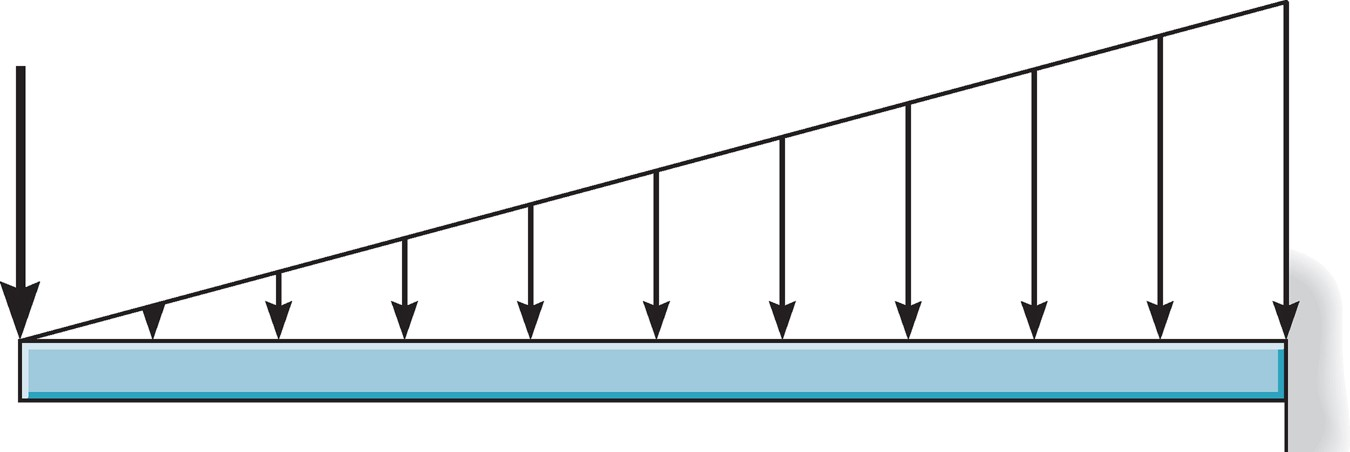
\includegraphics[width=0.6\linewidth]{p6-1f}
		\end{figure}
		\textbf{Solution:}
		\begin{figure}[H]
			\centering
			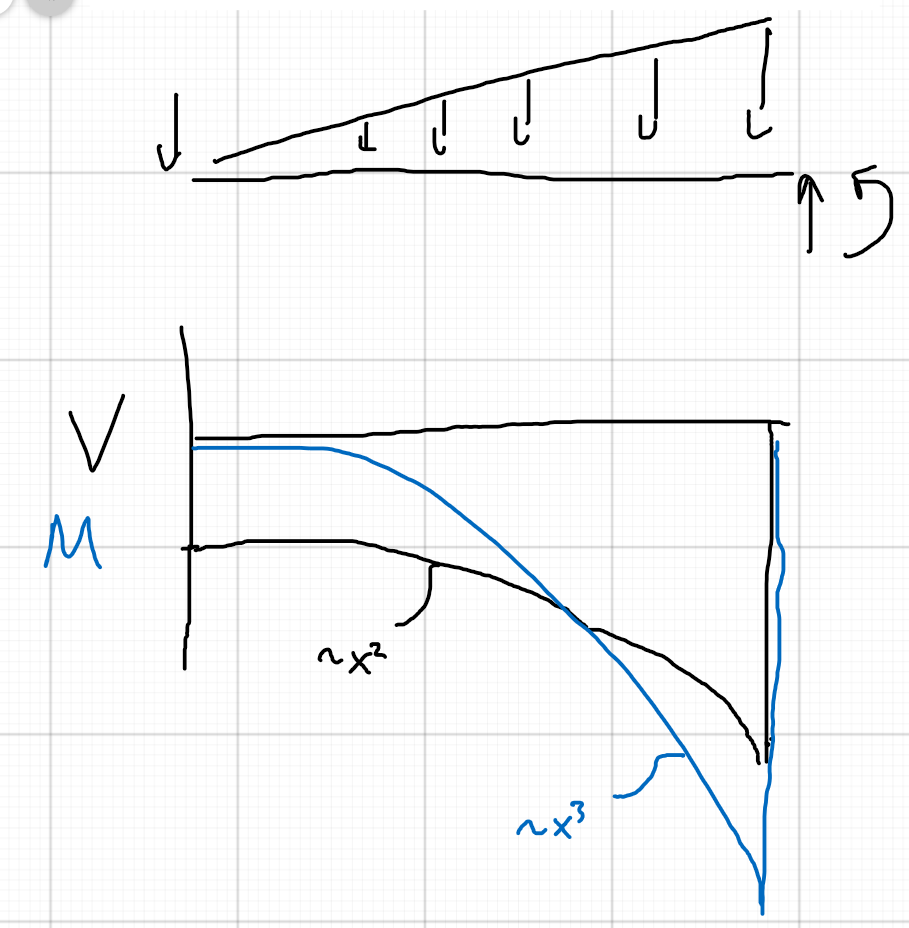
\includegraphics[width=0.5\linewidth]{5-1}
		\end{figure}

	\item %6-4
		Draw the shear-moment diagram for the simply supported beam
		\begin{figure}[H]
			\centering
			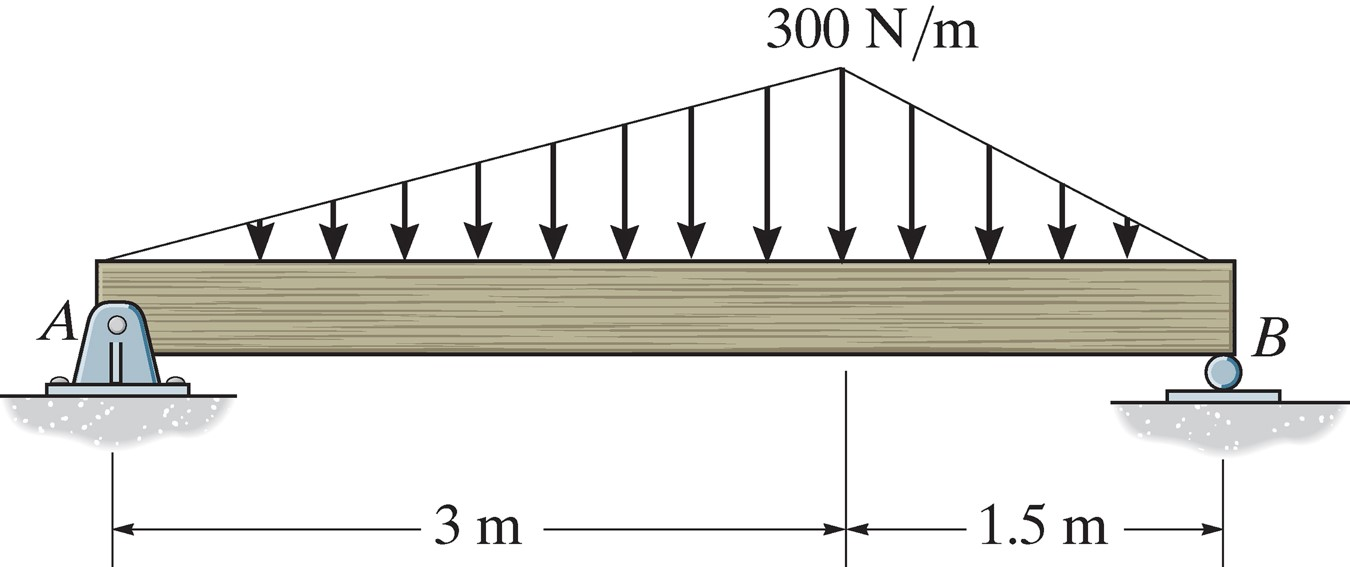
\includegraphics[width=0.6\linewidth]{6-4}
		\end{figure}
		\textbf{Solution:}
		\begin{itemize}
			\item We start by setting up a free body diagram to find the unknown support, $A$.
			\item NOTE: If we trust our process, we don't actually need to solve for $B$ (although once $A$ is found it is not difficult to do)
				\begin{figure}[H]
					\centering
					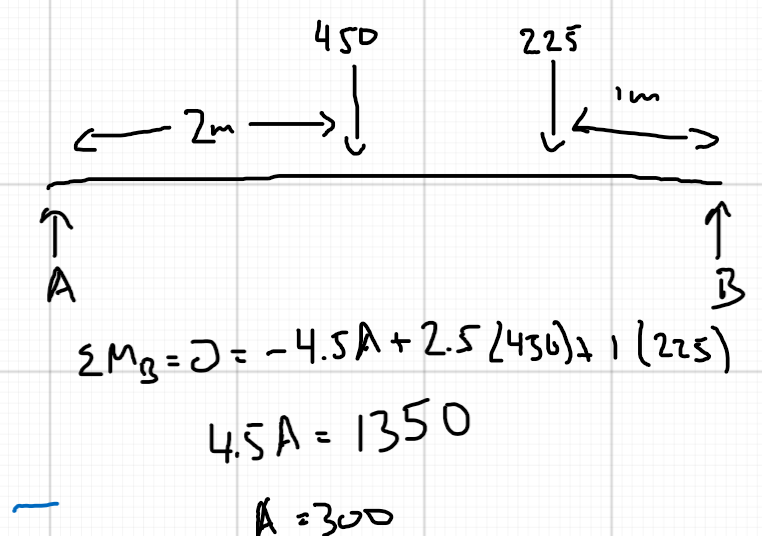
\includegraphics[width=0.6\linewidth]{5-2a}
				\end{figure}
			\item Now we have enough information to draw the general shape of the graph
				\begin{figure}[H]
					\centering
					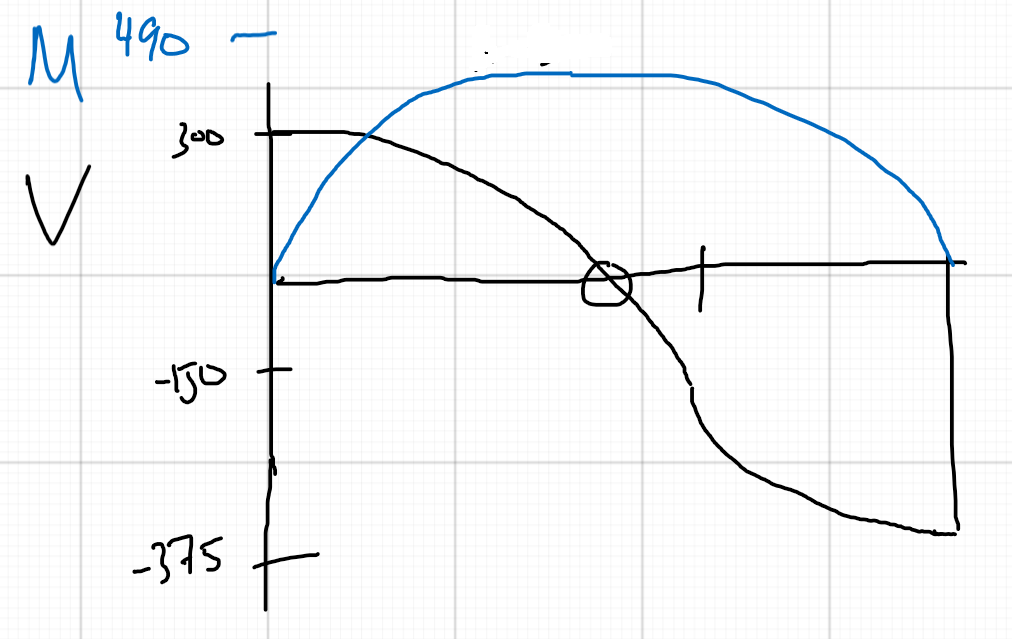
\includegraphics[width=0.6\linewidth]{5-2b}
				\end{figure}
			\item However, it is not obvious where the line crosses the $x$-axis, or the value of the maximum moment.
				To find both we section the beam and solve for $V(x)$ and $M(x)$ directly, but we need only consider the region near where the function crosses the axis.
				(This means we do not need to deal with a piecewise function).
				\begin{figure}[H]
					\centering
					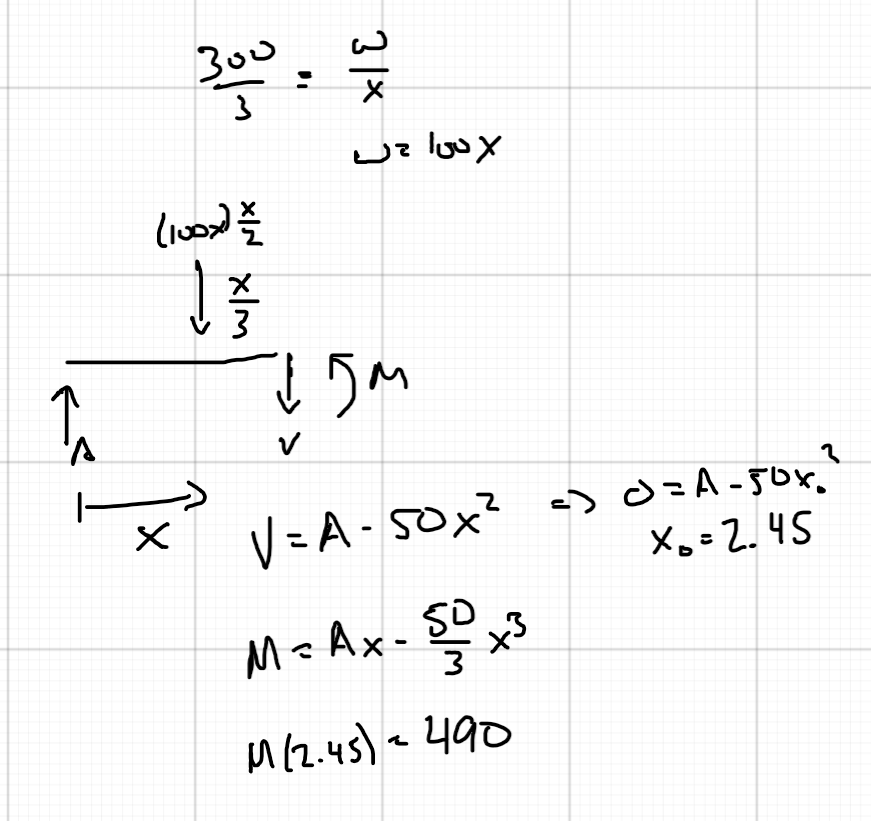
\includegraphics[width=0.6\linewidth]{5-2c}
				\end{figure}
		\end{itemize}

	\item %6-15
		Members $ABC$ and $BD$ are rigidly connected at $B$ while the smooth collar at $D$ is allowed to move along the vertical post.
		Draw the shear-moment diagram for $ABC$.
		\begin{figure}[H]
			\centering
			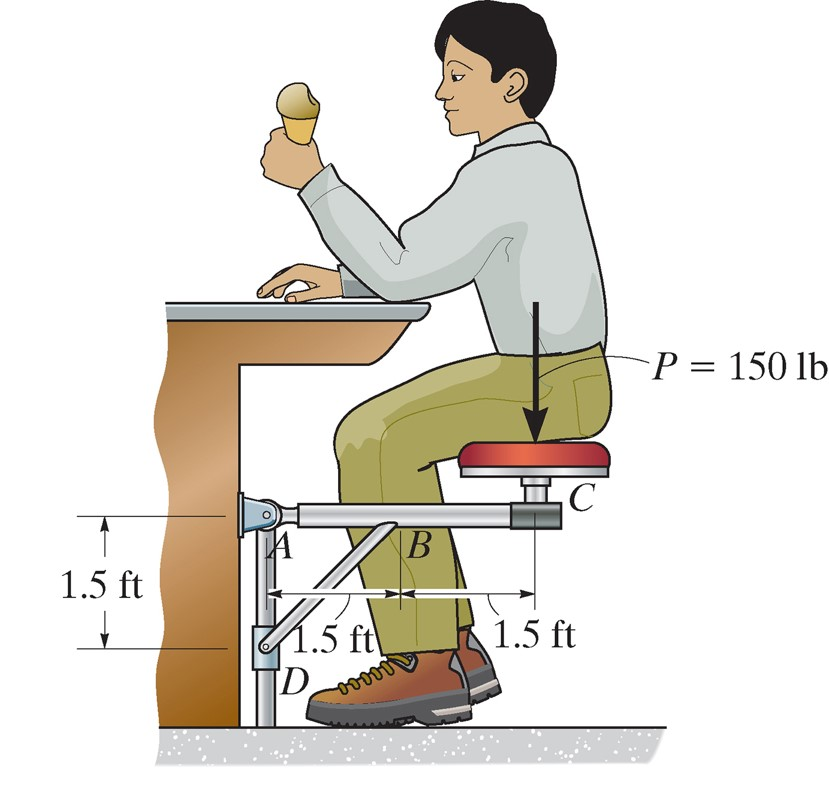
\includegraphics[width=0.3\linewidth]{6-15}
		\end{figure}
			\textbf{Solution:}
			\begin{itemize}
				\item There are possibly a few different ways to consider the free body diagram for this problem.
					Initially, I decided to use the rigidly connected portion.
					Notice that since the support at $D$ slides vertically (and is connected via a pin to allow rotation), it only exerts a reaction forces in the $x$ direction.
					\begin{figure}[H]
						\centering
						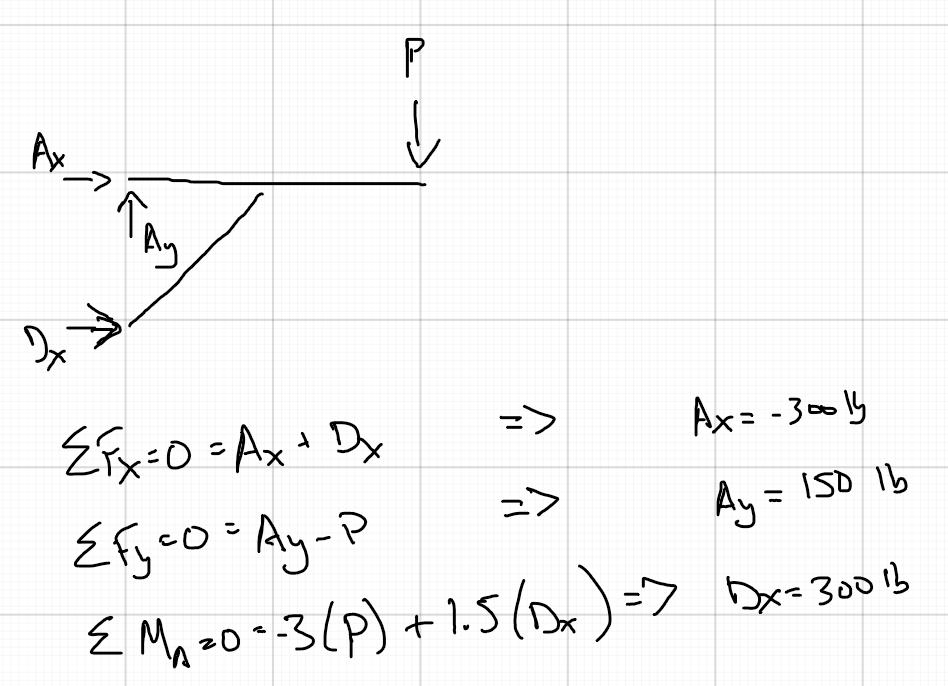
\includegraphics[width=0.6\linewidth]{5-3a}
					\end{figure}
				\item Since the problem asks for the shear-moment diagram of $ABC$, we need to remove the connection $BD$, to determine the internal forces at that section, I now considered a $FBD$ of $BD$
					\begin{figure}[H]
						\centering
						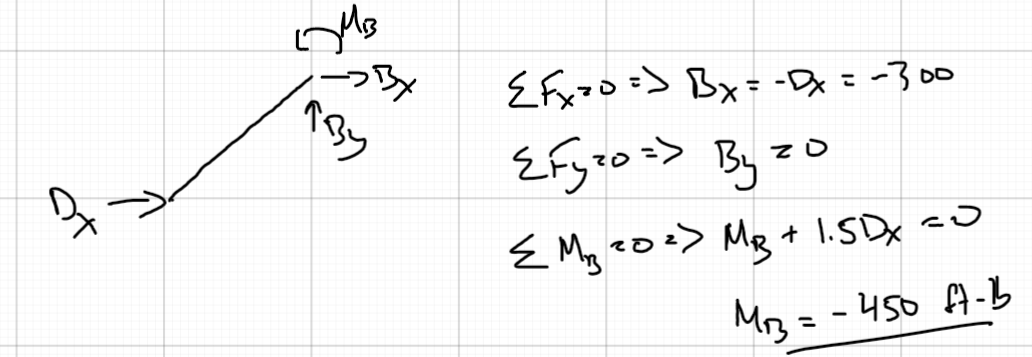
\includegraphics[width=0.6\linewidth]{5-3b}
					\end{figure}
				\item This gives the shear-moment diagram as
					\begin{figure}[H]
						\centering
						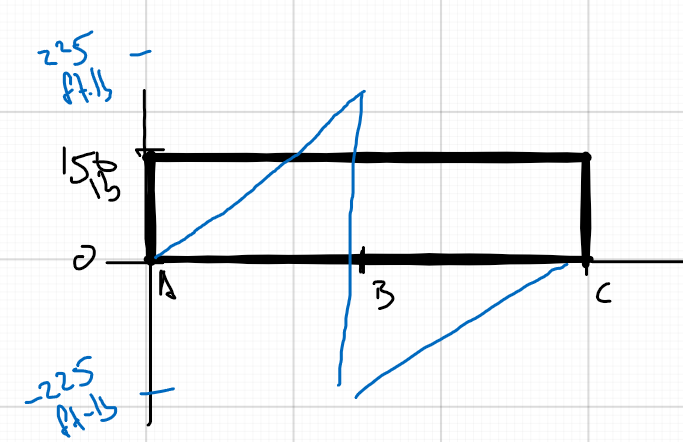
\includegraphics[width=0.6\linewidth]{5-3c}
					\end{figure}
			\end{itemize}

	\item %F6-12
		If the beam is subjected to a bending moment of $M=\SI{10}{kN.m}$ find the bending stress in the beam at points $A$ and $B$
		\begin{figure}[H]
			\centering
			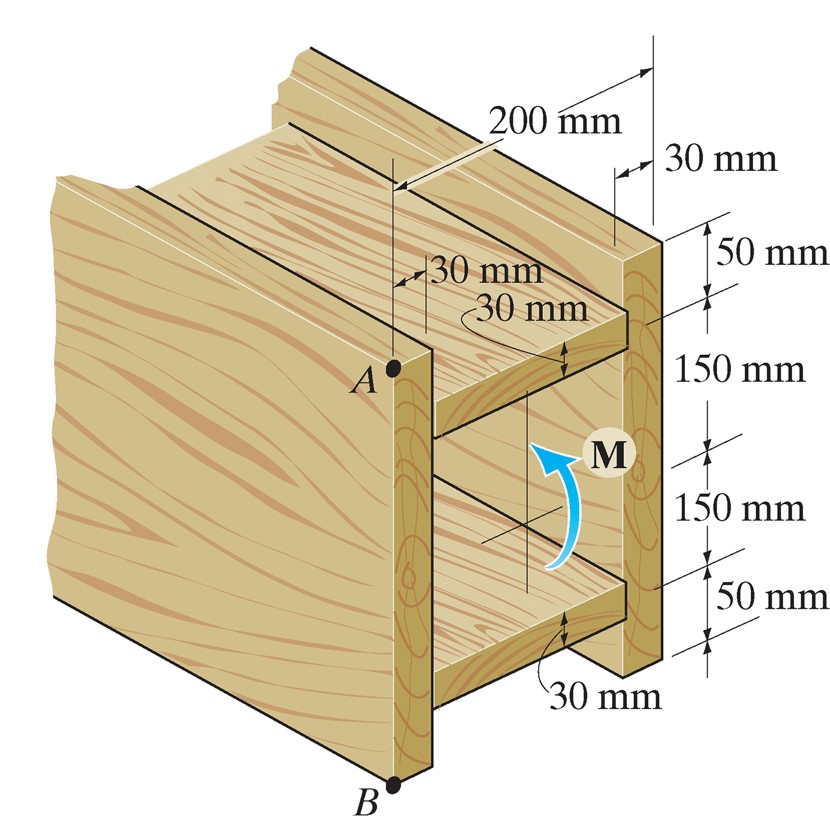
\includegraphics[width=0.5\linewidth]{f6-12}
		\end{figure}
			\textbf{Solution:}
			\begin{itemize}
				\item We will be using the flexure formula $\sigma = \frac{My}{I}$, since the moment is given we just need to find the neutral axis and the inertia
				\item The section is symmetric, so the neutral axis is simply the middle of the section
				\item Due to the symmetry we can find the total inertia as $I = 2I_1 + 2I_2$
					\begin{figure}[H]
						\centering
						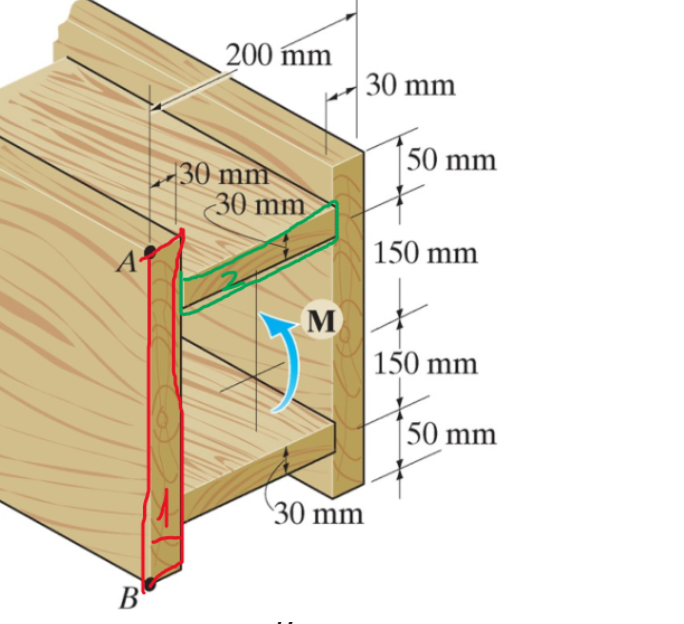
\includegraphics[width=0.4\linewidth]{5-4}
					\end{figure}
				\item This gives $I = 2\left( \frac{(30)(400^3)}{12} \right) + 2\left( \frac{(140)(30^3)}{12} + (140)(30)(150^2) \right) = 	\SI{509.6e6}{mm^4} $
				\item With $y = 	\SI{200}{mm} $ this gives $\sigma_A = 	\SI{-3.92}{MPa} $ and $\sigma_B = 	\SI{3.92}{MPa} $
			\end{itemize}

	\item %6-93
		Find the absolute maximum bending stress in the beam assuming that the support at $B$ exerts a uniformly distributed reaction on the beam.
		The cross section is rectangular with a base of $\US{3}{in}$ and a height of $\US{5}{in}$
		\begin{figure}[H]
			\centering
			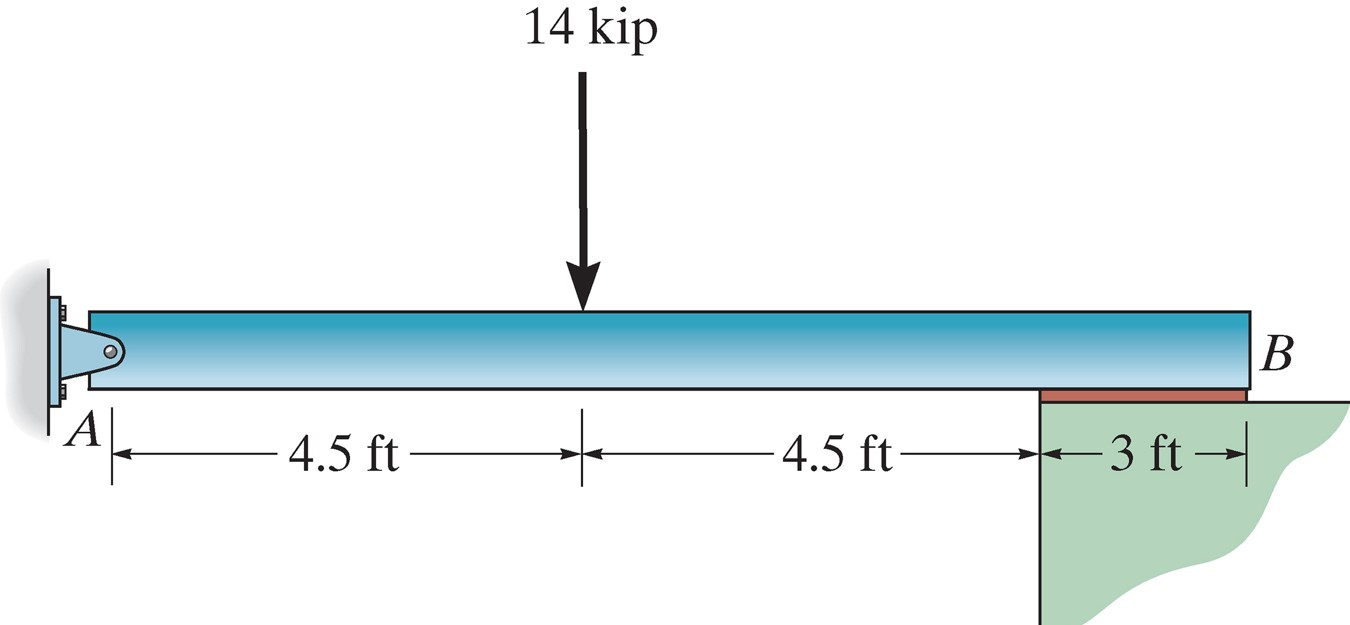
\includegraphics[width=0.6\linewidth]{6-93}
		\end{figure}
			\textbf{Solution:}
			\begin{itemize}
				\item To solve for the distributed load, we first treat it as a concentrated force located in the middle, giving the free body diagram shown.
					\begin{figure}[H]
						\centering
						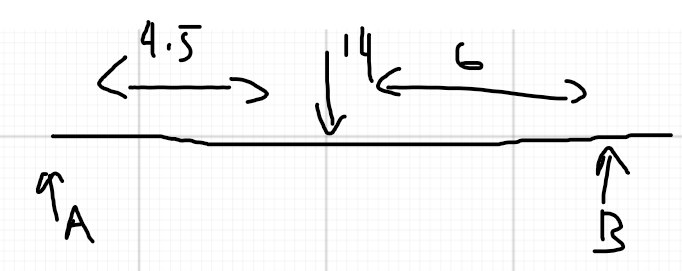
\includegraphics[width=0.6\linewidth]{5-5}
					\end{figure}
				\item We find $A = 	\US{8 }{kip} $ and $B = 	\US{6 }{kip} $
				\item The distributed load at $B$ is $ 	\US{6 }{kip} / 	\US{3 }{ft} = 	\US{2 }{kip/ft}  $
				\item We can draw a shear-moment diagram to find the maximum moment, which we need to find the maximum bending stress
					\begin{figure}[H]
						\centering
						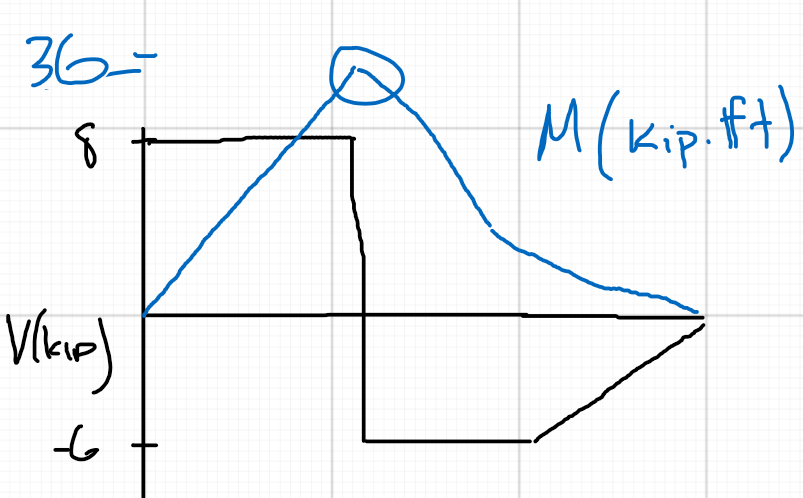
\includegraphics[width=0.6\linewidth]{5-5a}
					\end{figure}
				\item The inertia is just $I = \frac{(3)(5^3)}{12} = 	\US{31.25 }{in^4} $
				\item We find the stress $\sigma = 	\US{36}{kip.ft} 	\US{2.5 }{in} / 	\US{31.25}{in^4} = 	\US{34.6 }{ksi}  $
			\end{itemize}

	\item %6-101
		If the allowable bending stress is $\sigma_{allow} = \SI{6}{MPa}$, find the maximum dimension, $d$ of the beams cross sectional area.
		\begin{figure}[H]
			\centering
			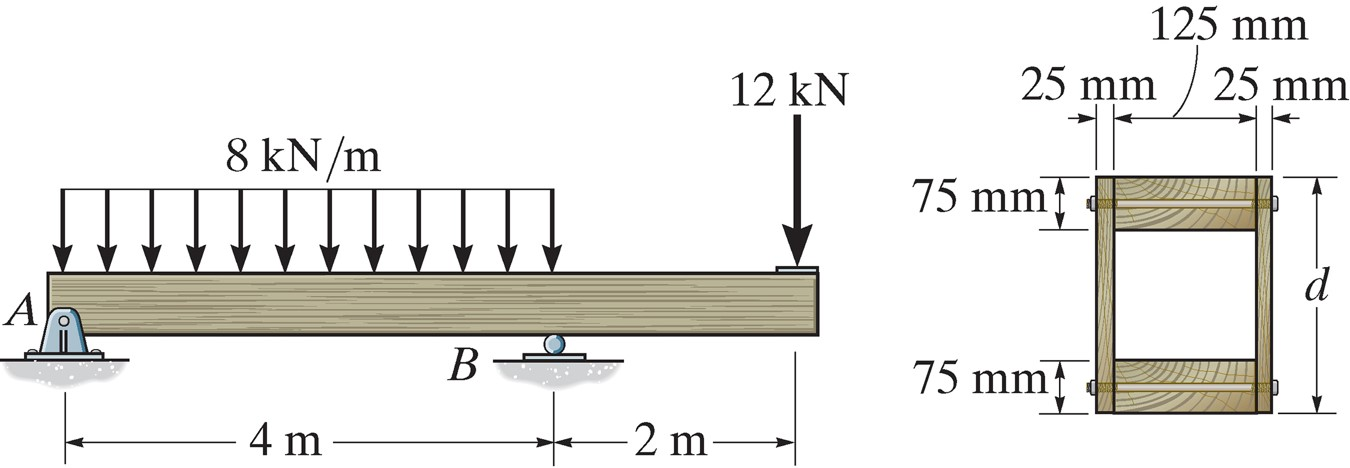
\includegraphics[width=0.8\linewidth]{6-101}
		\end{figure}
			\textbf{Solution:}
			\begin{itemize}
				\item We start by finding the maximum bending moment with the shear-bending diagram
					\begin{figure}[H]
						\centering
						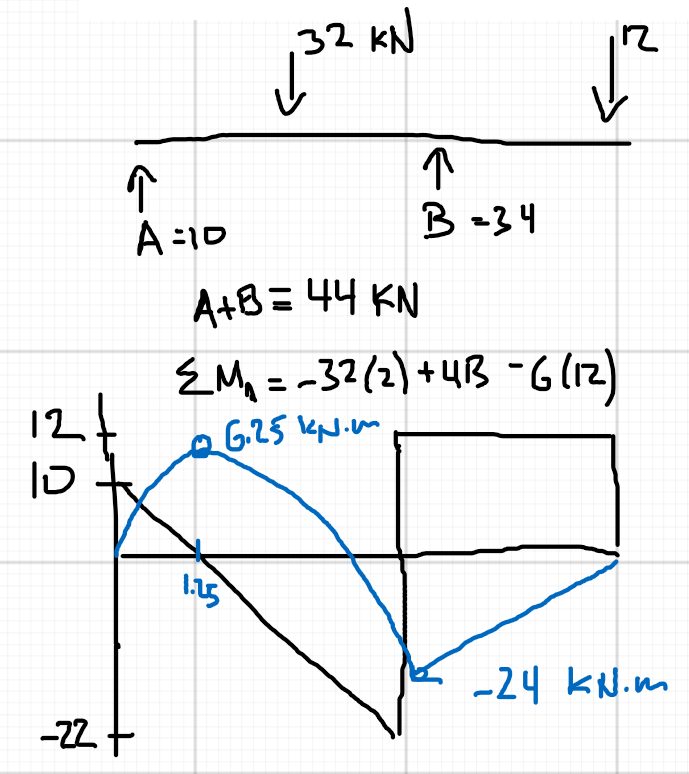
\includegraphics[width=0.6\linewidth]{5-6}
					\end{figure}
				\item We now need to find an expression for the inertia, $I = 2 \left( \frac{25d^3}{12} \right) + 2 \left( \frac{125(75^3)}{12} + 125(75)\left(\frac{d}{2} - \frac{75}{2}\right )^2 \right)$
				\item And finally we can set up an expression for $d$, $\sigma = 	\SI{6 }{MPa} = \frac{24 d/2}{I} = \frac{12 d}{25d^3/6 + 125(75^3)/6 + 250(75)(d/2-75/2)^2} $
				\item Before solving we need to make a note about unit consistency, since $\sigma$ is in MPa and our length units are in mm we need to convert the moment from kN m to N mm, we find $ 	\SI{24}{kN m} = 	\SI{24e6}{N mm}   $
				\item After simplifying, we find a cubic equation with three solutions for $d$, one of them is non-physical (negative), and we choose the larger of the remaining solutions, $d = 	\SI{409}{mm} $
			\end{itemize}

	\item %C6-4
		These garden shears were manufactured using an inferior material.
		Using a load of $\US{50}{lb}$ and appropriate dimensions find the maximum bending stress and show why failure occurred at this location
		\begin{figure}[H]
			\centering
			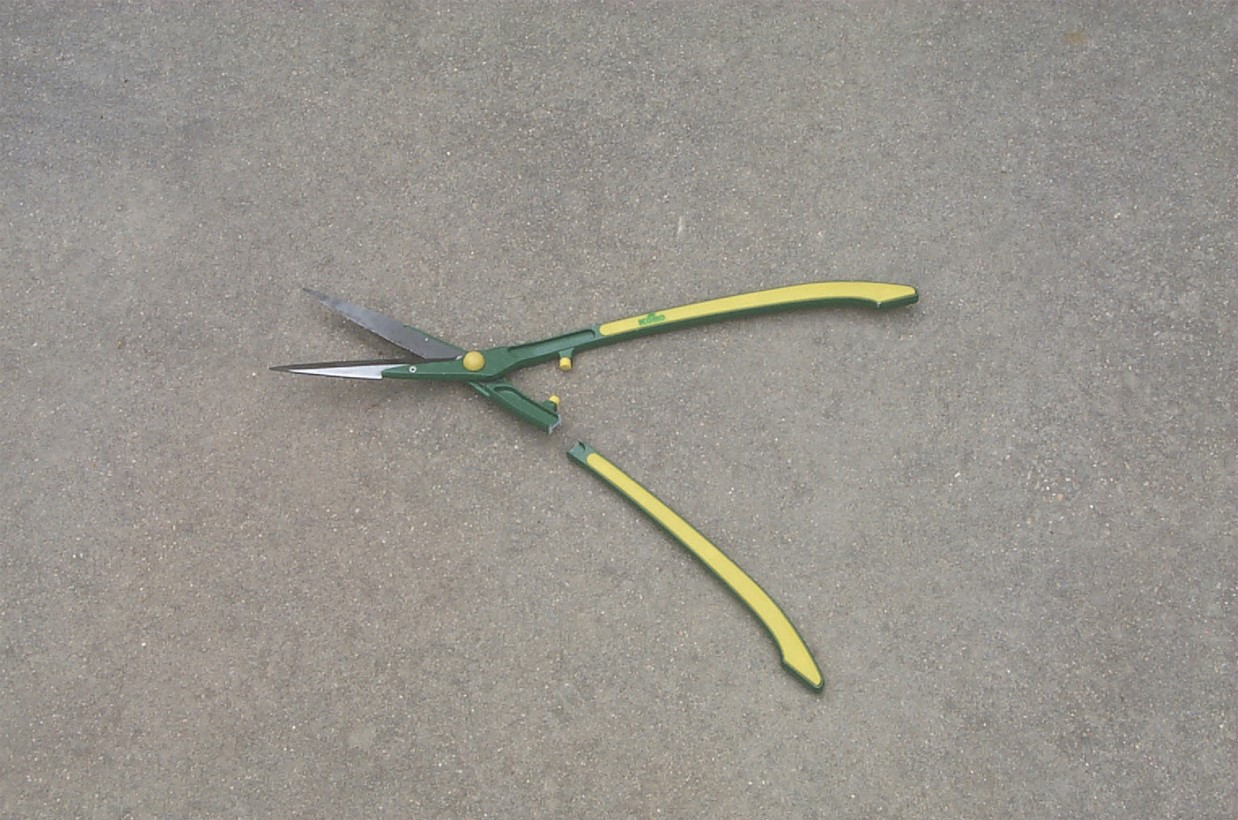
\includegraphics[width=0.7\linewidth]{c6-4a}
		\end{figure}
		\begin{figure}[H]
			\centering
			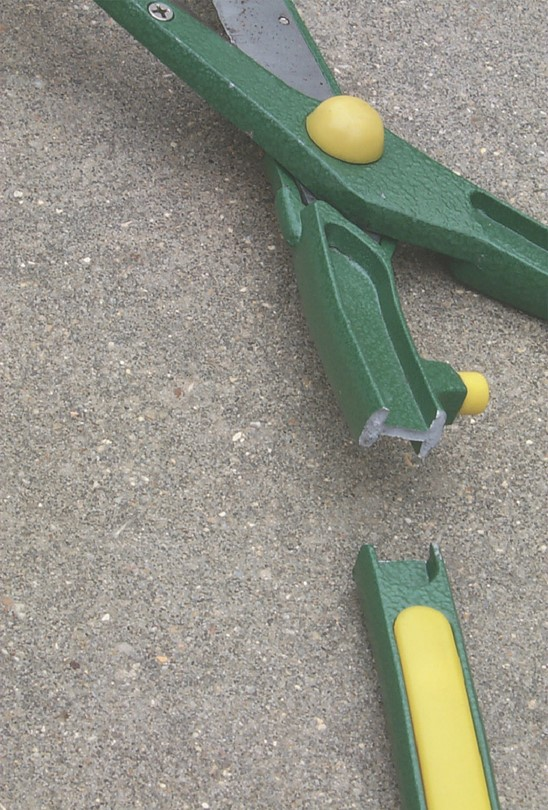
\includegraphics[width=0.4\linewidth]{c6-4b}
		\end{figure}
			\textbf{Solution:}
			\begin{itemize}
				\item It is actually unnecessary (and a bit difficult) to model the entire set of shears (and would depend on what is being cut), instead we can directly consider a handle section as shown
					\begin{figure}[H]
						\centering
						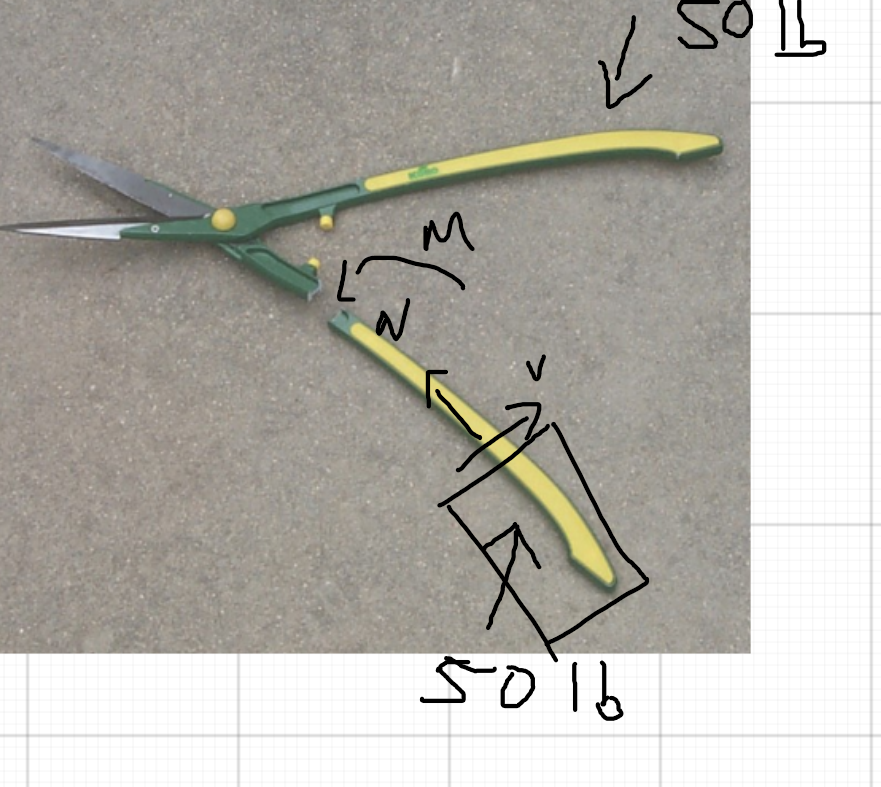
\includegraphics[width=0.6\linewidth]{5-7}
					\end{figure}
				\item We can see that the moment we find increases linearly until we reach the next support.
					Right at the point where the bending moment would be increasing to its maximum point, the cross-section also changes to decrease the inertia, $I$, which will also increase the stress.
				\item Assuming 3 inches of handle length between where we apply the load and the next support and an I-beam that is 1/2" tall, 1/16" thick and 1/4" wide in the I-beam flanges we find $I = 	\US{1.78e-3 }{in^4} $ and $\sigma = 	(\US{50 }{lb}) 	(\US{3}{in})( 	\US{1/4}{in}) / 	\US{1.78e-3 }{in^4} = 	\US{84.3 }{ksi} $
				\item This stress would be enough to cause failure in most steel alloys (and other metals) listed in the textbook, so clearly a heavier casting (with greater inertia) is needed to prevent this failure
			\end{itemize}
\end{enumerate}
\end{document}
